\chapter{Node communication and group state synchronization}
\label{chap:proto}
In this chapter we will be looking at some requirements and a suggested architecture for a protocol designed to facilitate group creation using the
distributed clustering algorithms discussed in the previous chapters. This protocol will be referred to as the Distributed Group Creation Protocol (DGCP).
While in the previous chapters the focus have been the algorithm for how groups can be formed and constrained, in this chapter the focus is on the technology and protocols required
to enable communication between access points and ultimately groups. There has already been done some work on the subject of access point communication over IP,
and previous work in the field of distributed consensus can be used to ensure synchronized group states. In this chapter these technologies will be covered and considered,
and finally a protocol sketch that stitches all required components together will be suggested. 


\section{Architecture}
In chapter \ref{chap:clustering} we looked at an algorithm that enables cluster formation in a distributed environment where no node knows the complete layout of the surrounding networks.
A number of assumptions were made before we suggested an algorithm. Two of the assumptions encapsulated the three following problems:
\begin{itemize}
\item Direct contact between access points is possible
\item An underlying group communication protocol is in place
\item The state of a group is synchronized throughout all its members
\end{itemize}
In this chapter we look at technologies that can handle these issues to suggest an abstract architecture for a protocol that enables group creation in a distributed environment.

\section{Enabling technologies}
When designing a protocol that enables group communication, it is good to have some already well-researched theory and technology as a foundation. There are enough
considerations to take when designing a new protocol architecture, and there is no need to reinvent the wheel in areas where there has been done a good amount of research. 
This section covers two technologies: Raft and ResFi. Raft will be used for state synchronization via log replication. It is a distributed consensus protocol and provides the equivalent degree of fault-tolerance as the Paxos \cite{lamport2001paxos} protocol family. ResFi is a protocol used to enable communication over IP between adjacent access points. 

\subsection{Distributed consensus with Raft}
Raft \cite{raftio} is a distributed consensus protocol designed with simplicity in mind. The creators of Raft designed it to be used for educational purposes. Traditionally, Paxos has been used to explain distributed consensus, but Paxos has a complex design with extremely many different variations. Raft is now taught in courses all over the U.S, and their GitHub page includes to links
of implementations in a large amount of languages. As Raft has such a wide range of implementations and is an easy protocol to understand relative to its quite complicated relative, Paxos, 
we will suggest that Raft will be used to handle distributed consensus. 

\subsubsection{Why distributed consensus?}
Distributed consensus is required for the distributed group creation protocol to provide data replication.
This makes sure all nodes have a consistent picture of the group, and in-case leader goes down any node is equally qualified to take on the role as leader.
The need for log replication is derived from the simple fact that there is no centralized controller to take decisions, so equally replicated data across all members node is required for all access
points to reach the same decisions about which neighbouring group to merge with, and also to compute channel distribution.  

\subsubsection{What Raft can not help with}
Raft is not originally intended to run in a flexible environment where the amount of servers changes rapidly. Thus, Raft is not able to handle the group membership changes
after two groups merge within the same Raft session. This is because there can be no consensus on past logs between nodes from different groups, as all groups will have different logs from before the merge. There is also no native Raft method to invoke native leader handover, so in the event of merge there would be two leaders. 

Another aspect that would be different from a traditional distributed consensus scenario, is the assumption that there are two main actors with different roles: servers and clients.
In distributed consensus, each server is supposed to have their own data, identical via data replication across across all the servers in the Raft session. The clients are the actor that requests 
changes on the data.

A traditional scenario is a banking example: a client could be a mini-bank issuing a withdrawal from a bank account. The servers would be all the banking servers making sure the new,
updated account balance is consistent no matter where money is withdrawn from. 

In a distributed group creation protocol all nodes running Raft are both servers and clients. They have to report new changes in the form of neighbours and signal strength values,
while also keeping a local, replicated copy of the state of the group.

\subsection{Access point communication with ResFi}
This subsection is dedicated to briefly describe how ResFi operates, and to cover why and how it is a protocol that can be taken advantage of in the Distributed Group Creation Protocol. 

As mentioned in the related work chapter at the beginning of the thesis, ResFi is a protocol framework that supports creation of radio resource management in legacy residential networks.
ResFi is intended to be used in a chaotically deployed landscape of access points, which is similar to the intentions of the group creation in this thesis. It enables the creation of secure point-to-point communication channel over IP through wired backhaul network. Point-to-point in this context means APs that are directly adjacent and can hear each other over the physical radio. ResFi also supports secure broadcast via n-hop communication. A brief account of the sequential steps of the ResFi standard mode of operation follows below. A more thorough explanation can be find in the ResFi paper \cite{resfi} under chapter \textit{IV. Detailed Specification}.

\begin{enumerate}
	\item When an AP ($a$) is booted, a symmetric group key is created, along with an RSA key-pair. 
	\item $a$ scans all 802.11 channels for neighbouring APs. For each AP it finds, $a$ sends out a probe request that contains its public IP and public RSA key. It also includes
		the symmetric group key. As a response to the probe request it receives a probe response containing the equivalent information for each neighbour. 
	\item When the exchange has happened, $a$ subscribes to the publish sockets of all the neighbouring nodes using the IP received in step 2. Each neighbour in turn subscribes to $a$'s
		publish sockets as well. This makes it possible for each AP to broadcast messages to all subscribed neighbours,
		or create a unicast session key between one specific AP to enable secure and bidirectional unicast communication.
\end{enumerate}

ResFi has a north-bound framework API that lets application running on the AP use ResFi's features through an API, without doing direct modifications to the implementation. All communication happens
in the JSON-format. Table \ref{tab:resfapi} shows which functions are available in the north-bound API, original table also including the south-bound API functions can be found in \cite{resfi} table 1.

\begin{table}[h]
	\small
	\resizebox{\textwidth}{!}{%
		\begin{tabular}{|l|l|}
			\hline
			sendToNeighbor(ap\_id, message) & \makecell[l]{Sends a message to an ap with id ap\_id. Message is in JSON format.\\The message is encrypted using the symmetric unciast session key.} \\
			\hline
			sendToNeighbors(msg, TTL) & \makecell[l]{Sends a message to all neighbours.\\Will be flooded out to n-hop neighbours, where n = TTL.} \\
			\hline
			getNeighbour() & List all neighbour AP IDs \\
			\hline	
			regCallbacks(newMessage, newNode, nodeDC) & \makecell[l]{Registers callback functions for the events new message,\\new neighbour node, and node disconnected. } \\
			\hline
			registerNewApplication(name) & \makecell[l]{Registers a new application with ResFi.\\Names are used to separate different applications.}\\
			\hline
			getResFiCredentials(param) & \makecell[l]{If param is 1, it return the public IP of the AP,\\ and if param is 2 it returns the public RSA key}\\
			\hline
			usePrivateRSAKey(data, mode) & \makecell[l]{Uses RSA key on tjhe data. If the mode is 1, it computes\\the signature of the data, if mode is 2 it assumed the\\data is encrypted and
																									decrypts it with the key.} \\
			\hline
		\end{tabular}}
		\caption{ResFi north-bound API}
		\label{tab:resfapi}
\end{table}


\section{Protocol}
This section outlines the architecture of a protocol that could facilitate group creation.

\subsection{Architectural overview}
The protocol architecture we suggest here relies on 4 main components which can be seen in figure \ref{fig:dgcpoverview}.
In the figure the blue boxes signifies logic that has yet to be implemented, while grey boxes signifies the components that needs to pre-exist. The arrows
represents which of the components that has to communicate with each other. In the next few subsections we address the two blue components individually.


\begin{figure}
	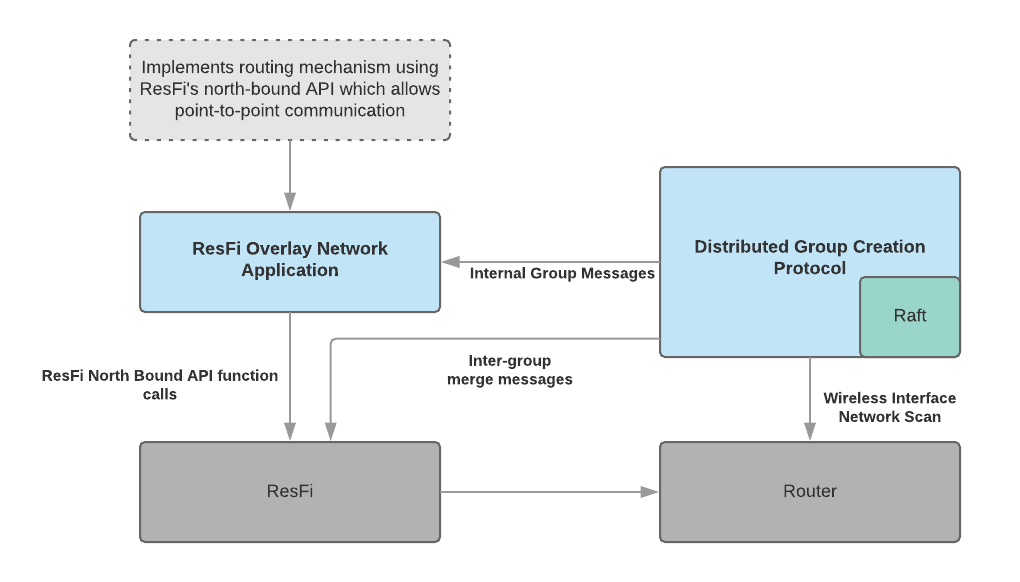
\includegraphics[width=\textwidth]{Images/dgcpoverview.png}
		\caption{Architectural overview of protocol components }%
		\label{fig:dgcpoverview}%
\end{figure}


\subsection{ResFi Overlay Network Application}
As made clear earlier, ResFi enables secure two-way communication between 1-hop neighbours, and broadcast messaging via n-hop neighbours. 
To enable secure two-way unicast communication throughout the group, an overlay network application can be built using the north-bound ResFi API. 
This means the overlay network application would have to use ResFi for point-to-point communication, and then implement its own routing mechanism
to relay messages from node to node, until the message reaches its destination. Let us look at the following suggested criteria for the ResFi Overlay Network Application:

\begin{itemize}
	\item Messages sent through the ResFi Overlay Network Application can only reach members of the group. If a message is requested for a node not inside the group,
		the message is not relayed.
  \item Should be used for all communication between nodes, like control messages, Raft log updates, etc., except for merge messages, which would have to happen across
		groups. 
	\item Needs a way to uniquely identify nodes to perform routing
\end{itemize}


\subsection{Distributed Group Creation Protocol}
This subsection is dedication to a suggested architectural overview of the Distributed Group Creation Protocol (DGCP). 
The protocol relies on the ability to directly interface with the access point radio, to execute and parse the results of the network scan. The protocol also
needs to be able to send message through the ResFi Overlay Network Applications to the rest of the group, as well as direct access to the ResFi north-bound API to be able to contact 1-hop
neighbours that are not in the group, to negotiate merges. 

The roles of a node running the protocol is illustrated in figure \ref{fig:dgcproles}. What follows is an account on the different services and functionalities the protocol
has to implement.  

\begin{figure}
	\centering
	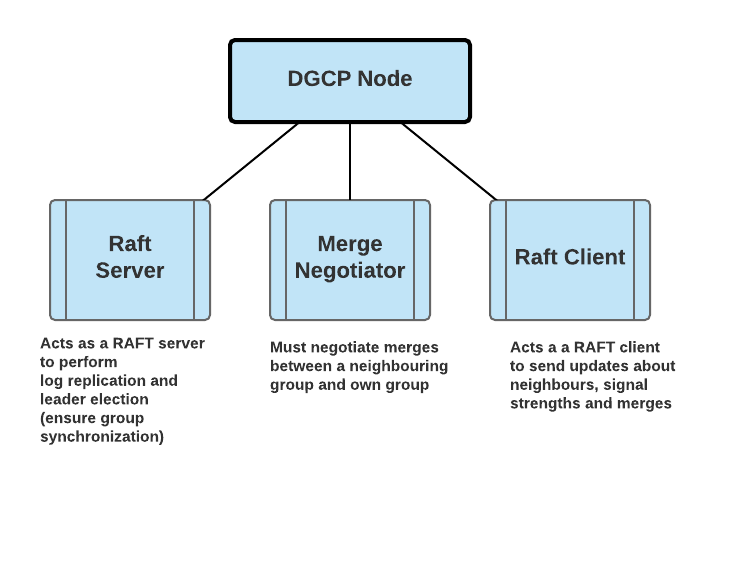
\includegraphics[width=8cm]{Images/dgcpnode.png}
		\caption{The roles of a DGCP Node }%
		\label{fig:dgcproles}%
\end{figure}

\subsubsection{Deciding which nodes to merge with}
Since the beginning of the thesis, the idea has been to let all nodes have the exact same information about the group state to calculate the same results. Deciding
which neighbouring groups to merge the group with is done by checking which nodes in the group has the most impactful neighbours. As all nodes in the group should share
the same information, all nodes will find the same result of which neighbour to merge with.
In the event that nodes in the group observe neighbours with exact equal signal strength, there will need to be implemented a deterministic way to decide which of the nodes would be chosen.
This could be as simple choosing the neighbours with the highest alphabetical order of the SSID. The important matter is that all nodes reach the same result of which group to merge with. 

\subsubsection{Negotiating merges via message passing}
We established that the protocol has to make sure all nodes in a group conclude which neighbour disturbs the most on their own.
The node that has this most significant disturber on their direct neighbour list, has to negotiate a merge for that node. 
This thesis will not address exactly how that message passing would look, but when a merge has been negotiated, and is either accepted, declined or a split is issued,
any changes of group membership to be reported to the Raft leader, so the updated group can be replicated to all members. 

\subsubsection{Internal group messages}
Group communication messages should include (but may not be limited to):
			\begin{itemize}
				\item Neighbour updates, e.g. a new access point appeared on the network scan of one of the routers, or significant signal strength value changes
				\item Raft log updates, heartbeats, vote requests, and vote messages
				\item Results of merges 
			\end{itemize}
				
\section{Assessment}
This chapter has introduced two pre-existing technologies that can help the process of building and implementing a group creation protocol. ResFi focused on the communication aspects between
neighbouring access points, while Raft has been suggested as a way to provide distributed consensus and data replication within the group. We have looked at the architecture that
would need to be in place to facilitate this protocol, and suggested some required functionality. 

We have not directly addressed what types of messages would have to be passed in the protocol, nor the data structure of the messages. The main reason for not addressing these large aspects is 
that the complexity could quickly become large, and it would exceed the scope of the thesis. It would be more fitting to address these topics when there is an intention of creation
a protocol implementation to be able to test a proposed architecture in its entirety.  

Hopefully it can be helpful as a starting point for a complete protocol architecture in the future. 

\chapter{Conclusion}

\section{Summary}
The premise of the entire thesis can be summarized in two points. 
\begin{enumerate}
	\item Performance of 802.11 residential Wi-Fi networks would be better if access points could collaborate on computing a channel plan
	\item There exists a computational limit to how many APs can collaborate, hence we have to identify which AP should be in the group with who
\end{enumerate}

Data and a data structure was needed to do simulations of the group creation algorithms. At the beginning of thesis we created the data structure
to be used for storing network topologies and group simulations. Instead of only using artificial data, we looked at WiGLE, an online web resource that gathers location information about access points from the entire world, and how to use their API to download data by specifying coordinates of interest.
To visualize the data as well as provide a way to step through each iteration of the group creation stage, we implemented a small web tool in HTML and JavaScript that parses the data.
It presents a visual representation topology, and an interface to step through it. This web tool has been used throughout the thesis to visualize the groups, separated by color. 

Furthermore, we began looking at how distributed clustering would have to happen to identify groups of hight impact nodes.
All nodes knows only the signal strength to their own neighbours to begin with, hence clustering decisions had to be made from each nodes point of view. Hence the bottom-up agglomerative 
hierarchical clustering was assessed, and modified to a slightly different algorithm that provided comparable results in a static environment. This algorithm lacked flexibility in-case of
topology changes or introduction of new nodes. To address these issues, we proposed two new algorithms, both with the same basis, but with an additional stage called splitting, where a group could split itself to allow for a more beneficial merge. One, using a modified version of K-means, another using the minimum cut theorem from graph theory. We used some real-world network topologies
to regard the cuts and to see if they were made in a reasonable place.  

Finally, we presented some relevant technologies that could facilitate a distributed group creation protocol, and presented an abstracted architecture of such a protocol.

\section{Discussion and contribution}
There are certainly many things to discuss and many challenges to overcome before a full-fledged solution for collaborative channel allocation can be performed.
In the related works chapter at the beginning of this thesis, we saw that there exists a large amount of centralized solutions
to optimize the performance of 802.11 Wi-Fi networks. But centralized solutions are single points of failures, and certainly very hard to deploy in residential networks where new
units may appear and disappear within minutes. Some solutions exists for residential areas, but they are more focused on coverage and other aspects of Wi-Fi. Like 
Google's routers utilizing mesh technology, and Domos routers who focuses on using AI to measure and evaluate QoS to give customers comprehensive diagnostic reports and improvement suggestions. 
None of these products help solving the fundamental issue: regaining control of the wireless spectrum. This is where this thesis picks up the thread. The value of the results in this
thesis lies in the proof-of-concept clustering that has been done. We have suggested a way to bootstrap clusters of nodes into groups, and respond to changes in the network topology
by group splitting. By creating such group we can look to previously created channel algorithms, like the channel algorithm from 2004, based on DSATUR. It does not address the
problem of limiting the amount of nodes to include in the coloring graph for channel assignment, but when combined with a group creation protocol it could possibly provide a new direction for
channel allocation in chaotically deployed Wi-Fi.  

\section{Future work}
There is a long road ahead to be able to perform the group creation in a real-life wireless topology. This section is dedicated to presenting some possible topics of research
that could further the vision of a decentralized, self-managing wireless AP topology. 

\subsubsection{Protocol development}
We briefly introduced an abstracted protocol architecture with relevant supporting technologies and data flow. Further development on this area would include a full protocol design, with
specified message types and data structures to be involved. An implementation of the protocol would be a natural next step, ideally with a testbed to confirm results. 

\subsubsection{Security assessment}
Is the ideas presented here possible to unify with great security? This is a question untouched by this thesis, and could provide another topic for future work. This should ideally
be done before or together with the protocol development. 

\subsubsection{Clustering assessment}
The clustering algorithms we developed and tried in this thesis may not be the ultimate answer. We have provided a proof-of-concept for how distributed clustering can be performed, and 
a comparative assessment between the methods, but no detailed evaluation of the quality of the clusters. There might different approaches to the distributed clustering problem 
posed in this thesis. A detailed assessment of the ones suggested here and other alternatives might be the basis for another thesis or further research.


